\subsection{Stability analysis}
\label{sub:a_}

The stability analysis of the jacobi solver did not converge to the
analytical value for increasing $\rhomax$, as this increased the step size
and caused reduced precision. For $N=200$, a $\rhomax$ of $\approx 5$ was
found ideal for the third wavefunction in the non interacting harmonic
oscillator. As seen in \cref{fig:rhoMax1} and \ref{fig:rhoMax2}, the
critical value for $\rhomax$ is  Then setting $\rhomax$ equal to 



\begin{figure}[H]
    \centering
    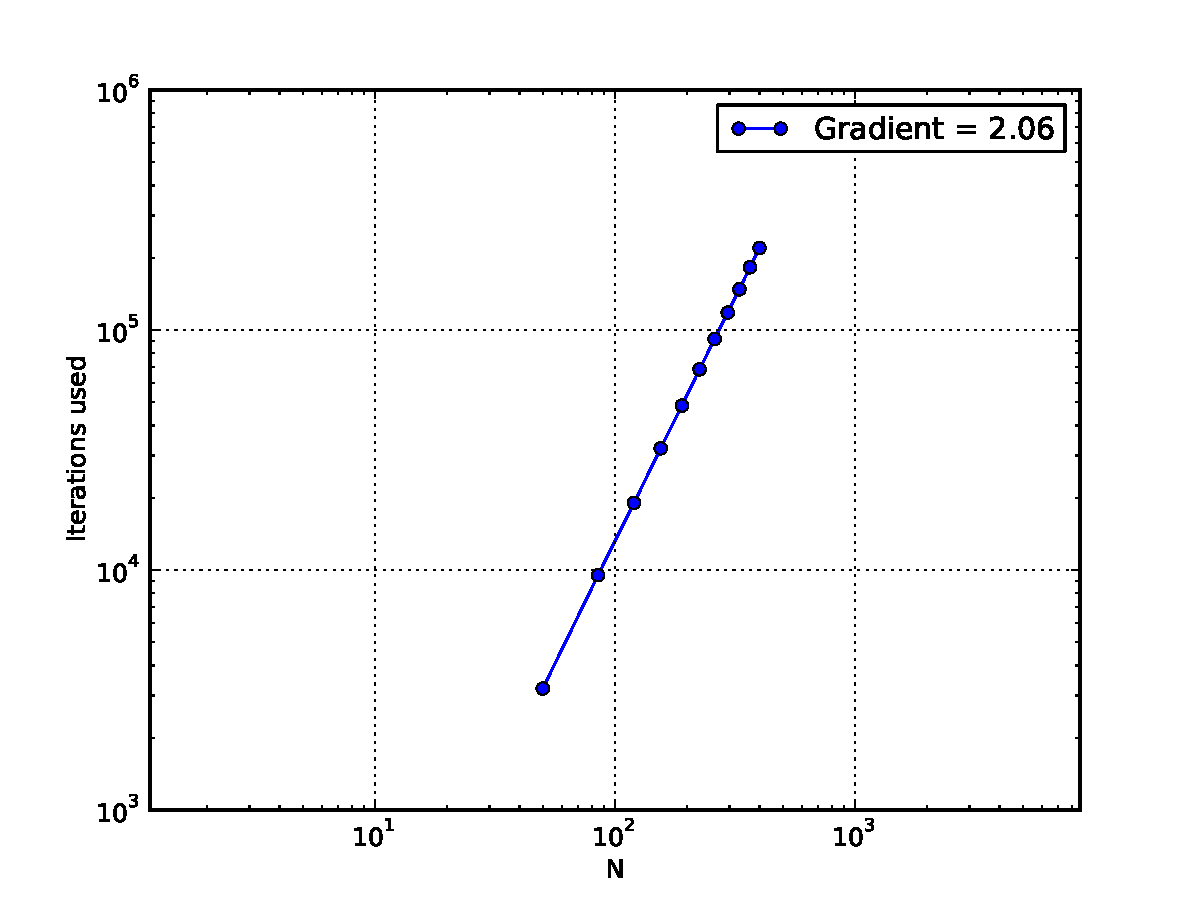
\includegraphics[width=0.8\linewidth]{iterations.pdf}
    \caption{Iterations of jacobi rotate vs N}
    \label{fig:iterations}
\end{figure}

\begin{figure}[H]
    \centering
    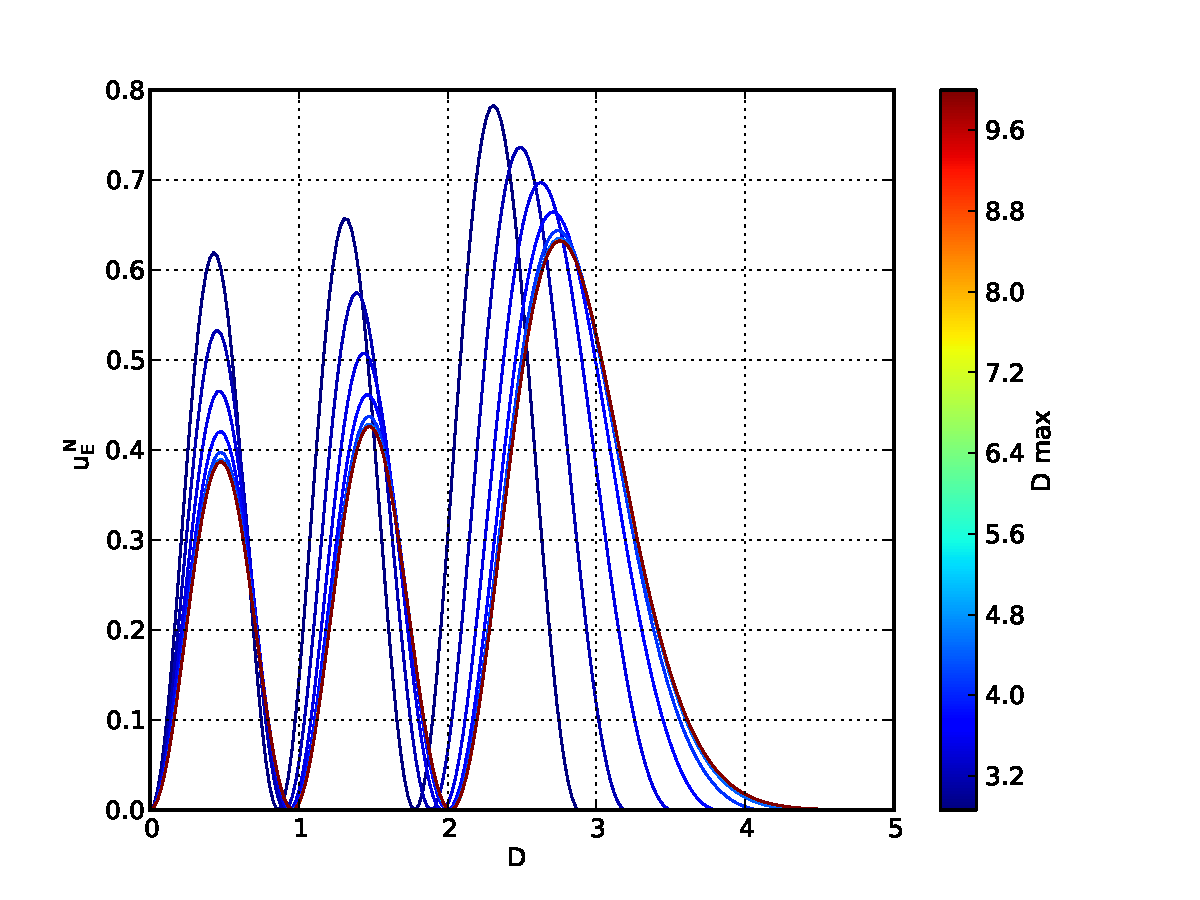
\includegraphics[width=0.8\linewidth]{rhoMaxAnalysis1.pdf}
    \caption{Convergence of $\rhomax$. As}
    \label{fig:rhoMax1}
\end{figure}

\begin{figure}[H]
    \centering
    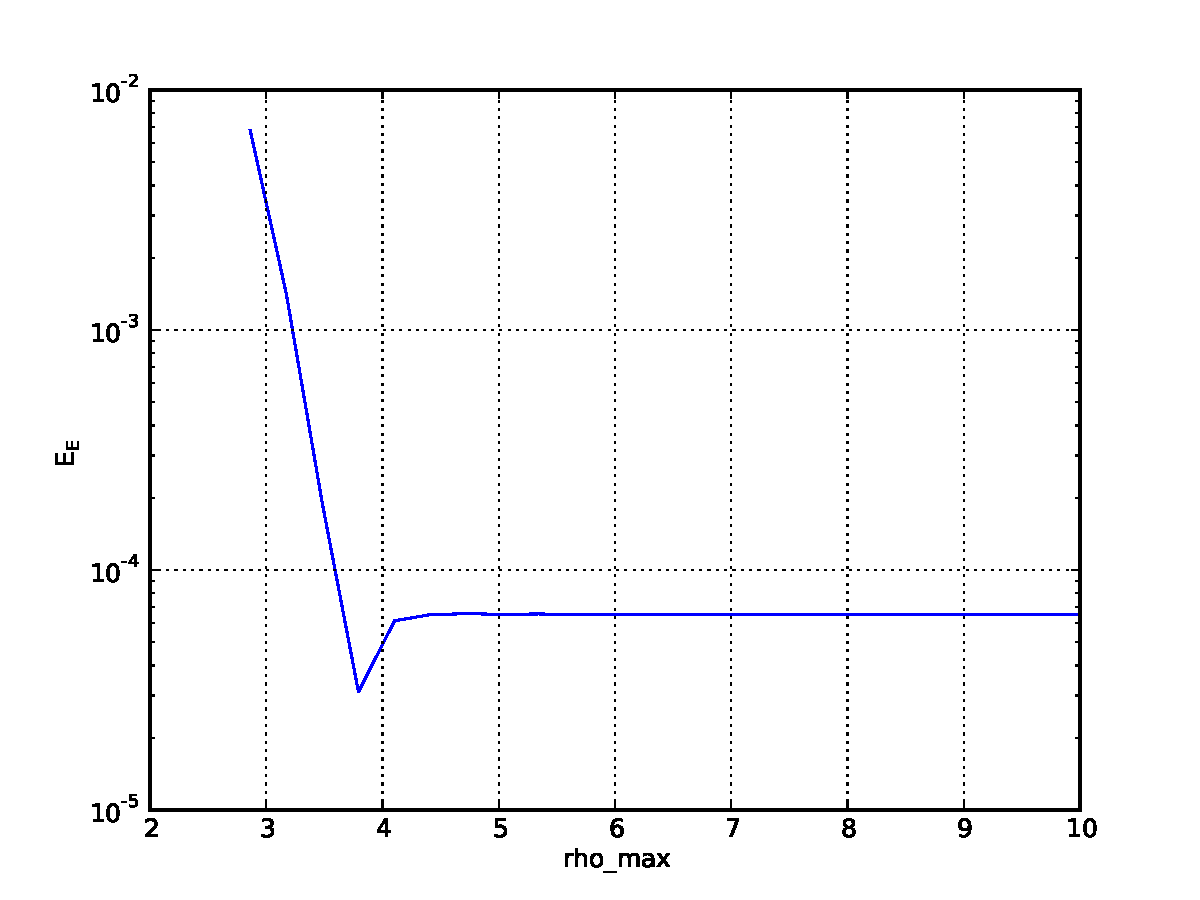
\includegraphics[width=0.8\linewidth]{rhoMaxAnalysis2.pdf}
    \caption{Convergence of $\rhomax$ }
    \label{fig:rhoMax2}
\end{figure}

\begin{figure}[H]
    \centering
    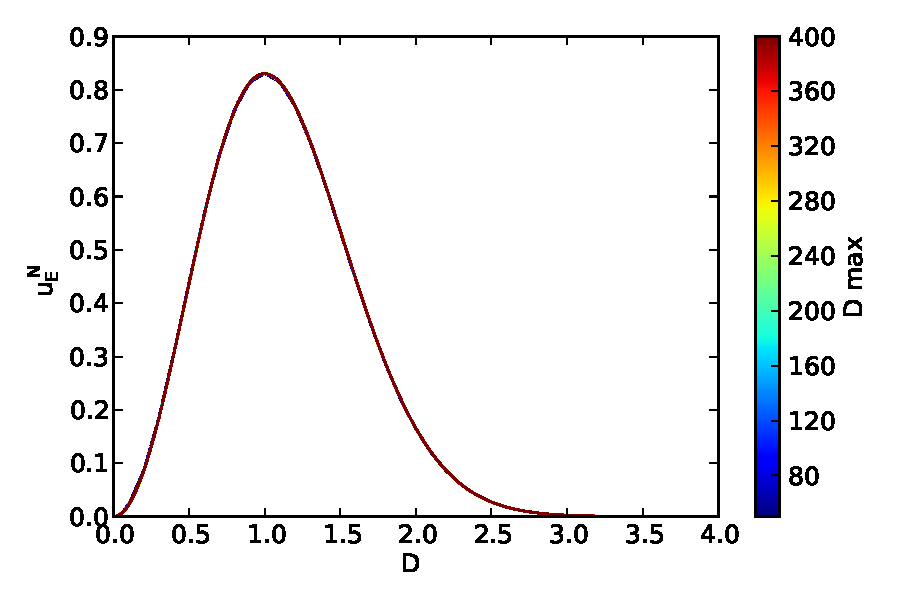
\includegraphics[width=0.8\linewidth]{dimAnalysis1.pdf}
    \caption{The normalized wavefunction in the testing the values of $N$.
    All values give visually similar wavefunctions.}
    \label{fig:dim1}
\end{figure}

\begin{figure}[H]
    \centering
    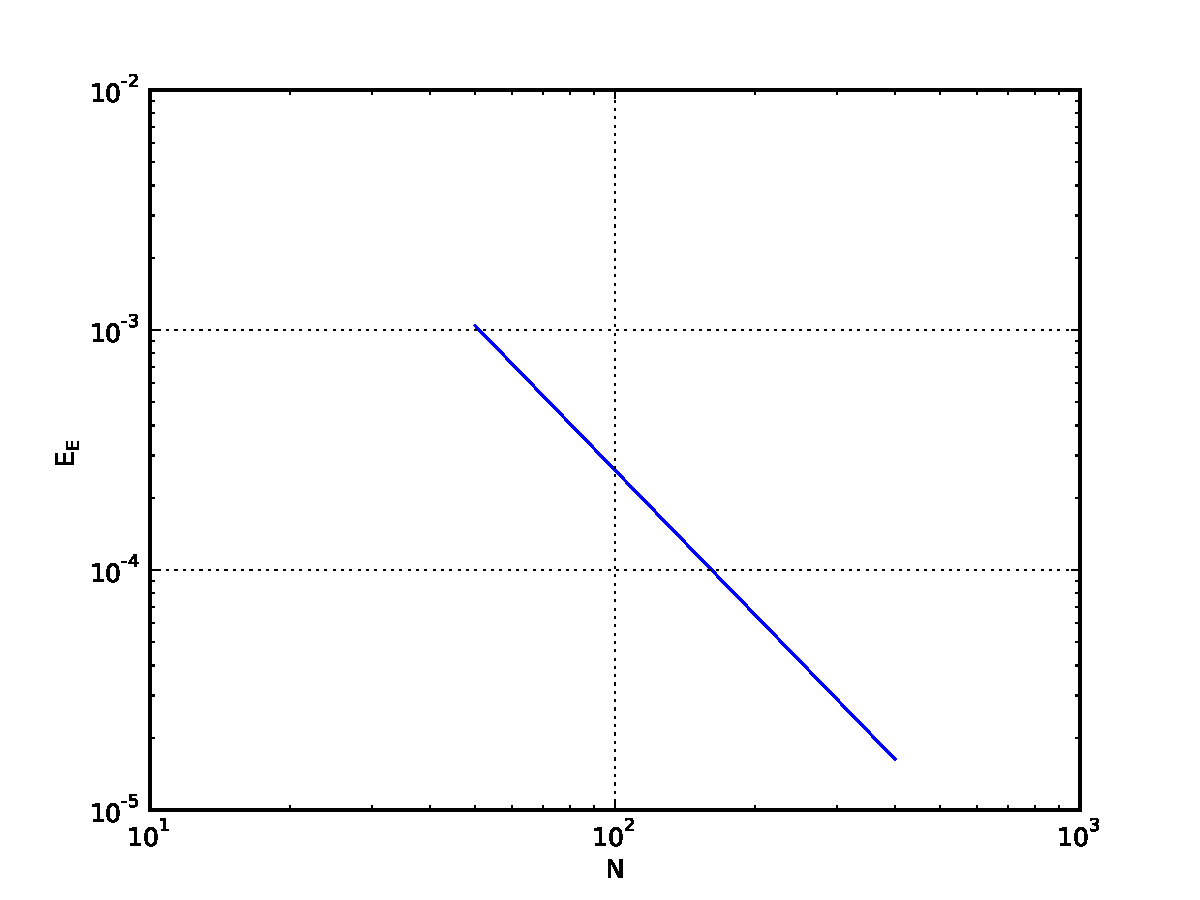
\includegraphics[width=0.8\linewidth]{dimAnalysis2.pdf}
    \caption{The normalized wavefunction in the testing the values of $N$.
    All values give visually similar wavefunctions.}
    \label{fig:dim2}
\end{figure}

\begin{figure}[H]
    \centering
    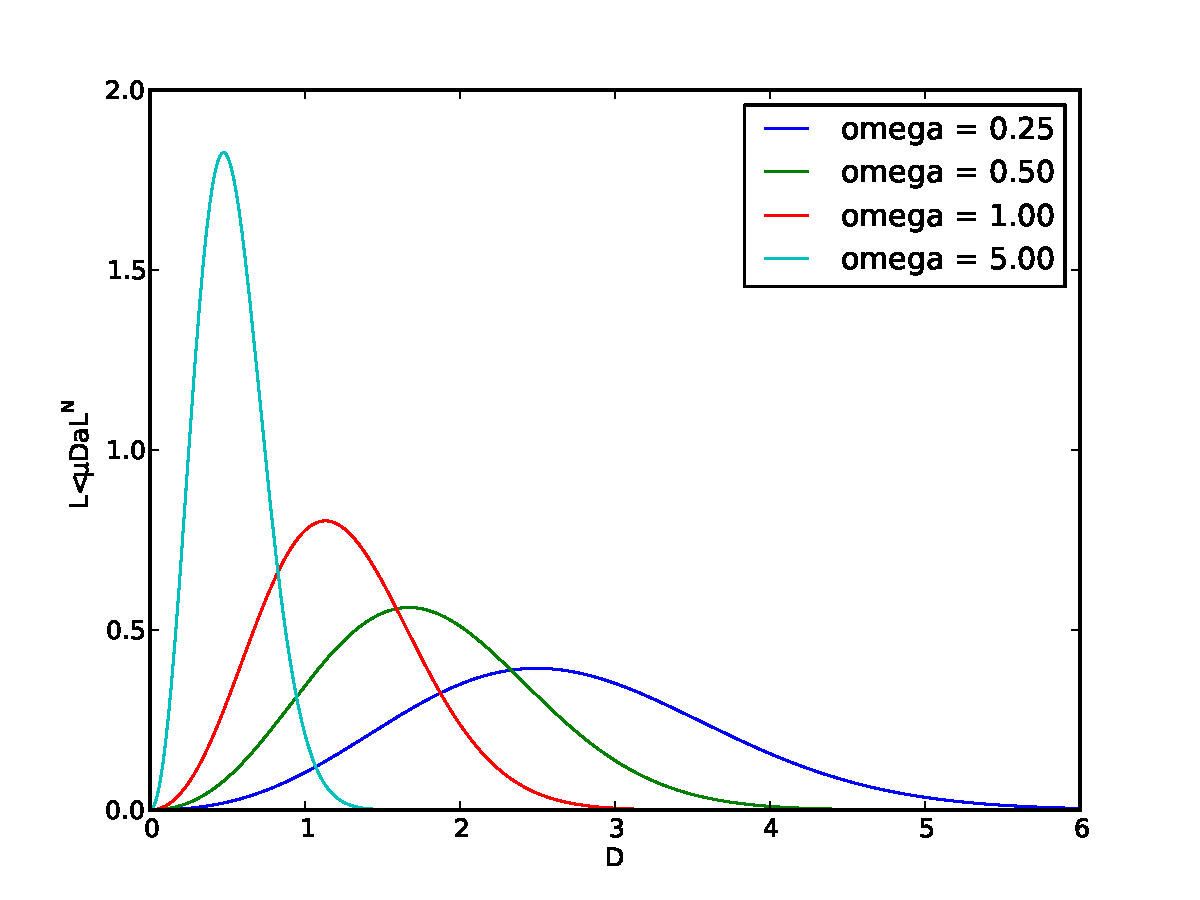
\includegraphics[width=0.8\linewidth]{waveFunc.pdf}
    \caption{Normalized wave function of the relative coordinate between
        the electron for the interacting case with $\omega_r \in\{0.25,
    0.5, 1.0, 5.0\}$.}
    \label{fig:waveFunc}
\end{figure}



